%%%%%%%%%%%%%%%%%%%%%%%%%%%%%%%%%%%%%%%%%
% Press Release
% LaTeX Template
% Version 1.0 (2/6/13)
%
% License:
% CC BY-NC-SA 3.0 (http://creativecommons.org/licenses/by-nc-sa/3.0/)
%
%%%%%%%%%%%%%%%%%%%%%%%%%%%%%%%%%%%%%%%%%

%----------------------------------------------------------------------------------------
% PACKAGES AND OTHER DOCUMENT CONFIGURATIONS
%----------------------------------------------------------------------------------------

\documentclass[11pt,pressrelease]{newlfm} % Font size

\usepackage{etoolbox}
\makeatletter
\patchcmd{\@zfancyhead}{\fancy@reset}{\f@nch@reset}{}{}
\patchcmd{\@set@em@up}{\f@ncyolh}{\f@nch@olh}{}{}
\patchcmd{\@set@em@up}{\f@ncyolh}{\f@nch@olh}{}{}
\patchcmd{\@set@em@up}{\f@ncyorh}{\f@nch@orh}{}{}
\makeatother

\usepackage{charter} % Use the Charter font for the document text

\PhrPhone{Phone} % Customize the "Telephone" text
\PhrEmail{Email} % Customize the "E-mail" text
%\PhrContact{Contact} % Uncomment this line to change the 'Contact:' text

%----------------------------------------------------------------------------------------
% PRESS RELEASE INFORMATION
%----------------------------------------------------------------------------------------

\makeletterhead{Uiuc}{\Cheader{\vspace{16pt}
\includegraphics[width=0.3\linewidth]{TSF_Logo_NB.jpg}}} % Include a company logo, if you don't use one you will need to uncomment line 6 in the prsrls.tex file
\lthUiuc % Print the company/institution logo

\release{For Immediate Release to Tartan Student Fund} % When the press release may be used

\namefrom{David Hiles, Head of Equity Strategy Team} % Name

\phonefrom{732-796-8352} % Phone number

\emailfrom{dhiles@cmu.edu} % Email address

\headline{Fall Portfolio Updates} % Headline for the press release

\newcommand{\subtitle}{This is a subtitle to the headline giving more information about the headline.} % Subtitle for the press release, if you don't want one just remove the subtitle text leaving the rest of the command

\byline{\textbf{Carnegie Mellon University -- \today ~--} A portfolio review for each sector group.} % A summary line for the press release

%----------------------------------------------------------------------------------------

\begin{document}
\begin{newlfm}

%----------------------------------------------------------------------------------------
% PRESS RELEASE CONTENT
%----------------------------------------------------------------------------------------

%\vspace{-.25 in} %.65 is normal
\begin{singlespace} % Uncomment for single line spacing
Since my last major publication in October of 2016, the TSF Portfolio is up 10.4\%. As we continue to recruit new talent and refine our processes I hope this trend will continue. However, the S\&P 500 is up a considerably more, showing a return around 18.5\% in the same period. As a quick aside, we are not fully invested and should not expect to match the index completely; when adjusting for the cash drag, the S\&P has returned 16.1\%. Our portfolio has a similar Beta to the overall market, due to our similar sector allocation. I have attached a chart outlining our underperformance compared to the large cap index. %While a discussion on overall valuations will follow, I would remind individuals to re-examine the concept of ``Margin of Saftey'' given current levels in most markets.

\begin{enumerate}
\item \textbf{Consumer Discretionary \& Staples} \par
This year, returns on our Consumer portfolio have been very positive and our outlook is positive as well. Our single name selections of \textbf{Nike} and \textbf{Kraft Heinz} have lagged the overall industry, but carried by the ETF's, the group has had solid performance over the year. Our \textbf{Nike} position has continued to weigh on the portfolio despite the trim in late 2016 and has been range-bound for almost 18 months now. As per the broader investment themes, \textbf{Nike's} sales growth and projected sales growth has not kept up with the broader sector and investors have been cautious about ``just doing it.'' As a group, I would recommend a revaluation of the \$KHC thesis, particularly the revenue growth catalysts. Both the Consumer Staples and Discretionary ETF’s have preformed well, although one would attribute this to the high correlations to the S\&P index. Our outlook moving forward varies per industry sector but with personal incomes rising (supplemented by record amounts of household credit), we may see further earnings growth in consumer businesses. %Sensitivity to rates is a concern moving forward. Nike correlation with rates

\item \textbf{Healthcare} \par
Sales and expansion has been the name of the game for 2017, with profitability taking a backseat for now. The sales growth has pushed individual names higher but the overall Health Care index has stagnated. The HC index is trading around 25.5x and has struggled to break the mid 2015 valuation (31x TTM Earnings). Our two pharmaceutical related positions \textbf{Gilead} and \textbf{McKesson} have not recovered to their previous highs due to pressure on drug prices. Gilead has recovered through the summer due to new developments in their storied cancer related treatments, but remains a 20\% loss in the portfolio. Fundamentally, McKesson remains a strong player in the drug distribution space and we believe our thesis still holds. Like a handful of TSF picks in the past, we were incredibly skilled at buying companies at their 2 year highs and thus the \$MCK position is down 21\%. Our healthcare portfolio has been one of the hardest for us to manage, but our current holdings are buoyed by our large position in \textbf{United Healthcare} (up 23\% since March) and the strong performance of the \$XLV exposure.

\item \textbf{Financials} \par
The financials portfolio is our strongest performer with \textbf{Visa} proving to be our best preforming conviction pick in the entire fund. The other main story for the sector is the outperformance of \$VHF, benefiting greatly from the 2016 US Election. While \textbf{Fifth Third Bancorp} has performed inline with other regional banks, our timing missed much of the ``Trump Bump'' this sector enjoyed through early November of 2016. We remain cautious of this sector's dependence on regulatory change, but earnings have been promising and CCAR told us a significant amount regarding bank's balance-sheet health and well-being of financial systems in general. We still believe major banks could be undervalued compared to the S\&P and would recommend looking for companies that would benefit in the backdrop of rising rates.

\item \textbf{Power \& Utilities} \par
The PU group has rebounded strongly through the year, primarily due to a slight rebound and stabilization of oil and gas prices. With supply-demand dynamics in the crude markets stabilizing, management teams have cut CAPEX in many Exploration and Production companies, a necessary precaution for many of these firms. Thankfully, we have been underweight E\&P for most of the fund's history. Our Midstream and Downstream positions in \textbf{Spectra Energy Partners} (Midstream MLP) and \$PSX (Refining and Marketing) have preformed well, and wider crack spreads has allowed refiners to maintain solid revenue figures and expand operations. With respect to utilities, we find the bond proxy theme has held through most of 2017. With real yields lower than expected, utilities with the highest (yet slower-growing) dividend yields are near historical valuation peaks. Again, we want cash producing, strong dividend businesses from this group moving forward. \$DUK has performed in line with the broader ETF (\$XLU), both up roughly 17\% YTD. Companies with lower dividend yields and higher earnings growth are near attractive valuation levels at this time.

\item \textbf{Industrials \& Materials} \par
The promise of infrastructure spending has boosted these sectors to cycle highs. However, we are wary that this could be speculator inflows to the sector and we have maintained a diversified exposure to avoid idiosyncratic risks. While we currently have no conviction picks in this group, we have seen our ETF (\$XLB, \$VIS) positions up almost 30\% since last October. We are looking for businesses that are not dependent of rising commodity prices, as we do not have confidence in the commodity significantly rebounding. This is mainly due to slower growth in commodity producing emerging markets and the impacts of currencies.

\item \textbf{Tech, Media \& Telecom Group} \par
Our TMT portfolio has also performed well this year, driven by the sector's strength in the past nine months. We have allocated away from Telcom in this portfolio, which has proven to be an effective. Since the funds reorganization, we have maintained exposure to the \textbf{PowerShares Dynamic Media ETF} which has had disappointing returns versus the sector and broader market. The TMT group has positioned a portfolio of relatively cheap stocks for this stretched sector, with a 13.8 P/E (TTM). In recent developments, AT\&T missed earnings in Q3 and investors are worried about the lack of synergies with the DirectTV merger completed last year as well as shrinking mobile subscribers. The stock has seen a volatile 19 months in our portfolio and we should be looking to re-evaluate our thesis moving forward. Like a few of our other portfolio groups, our clear winner in the TMT portfolio is the ETF, \$IYW. It's slow advancement to record highs was driven by a demand for growth stocks in information technology as well as the the ``FANG'' outperformance this year.

%\vspace{12 pt}

\center \textbf{Summary} \par
\raggedright
With current EPS (TTM) for the S\&P 500 at around \$104.02 /shr, a 30 year historical P/E ratio should only support a index value around 2,350. This was accomplished in May of 2017 and the market has since edged higher while volatility has fallen to historic lows. We believe that this market could be pushed further given that low real yields to support higher than history steady-state PEs across the markets. The expectation of tax cuts and possible cyclical acceleration have weighed heavily on certain sectors, further driving returns and allowing valuations to be stretched. Looking at the fund's history, the biggest market moves have been in Technology and Consumer Stocks. All other sectors have entered some sort of ``Bull Market'' since 2014, in what is most likely a pattern of sector rotation. Besides sharp corrections in from December 2015 to January 2016 (-14\%), Technology and Consumer Sectors have followed (and driven) the wider trend of the bull market in the past 3-4 years. %Taking a page from Dalio's Economic model, we largely attribute this to unprecedented household credit growth, while maintaining lower than average debt services levels. Takeaway? Without a widescale systematic event, we could continue to see this economic expansion continue past 2018 into 2020.

Investors in the past year have been much more concerned with sales growth and forward sales growth. Many value funds have underperformed the broader market, as investors look to buy disruptive businesses, at the expense of today's profits. We see some other evidence in the value vs. growth tilt: the Russell 1000 Value Index has returned 9.7 percent in the first 10 months of 2017, while the Russell 1000 Growth Index has gained 24 percent. We expect this trend to continue so long as yields stay low and thus the equity risk premium can compensate investors adequately. With accommodative rates, decent earnings and the (overly?) optimistic ideas of tax cuts, de-regulation and fiscal spending, we can anticipate stocks to keep crawling upwards. Many consider the current valuations uncharted territory, but in 2017 we are seeing earnings ``catching up'' to support current levels, despite a gradual tightening environment. Again, we are not hesitant in U.S. Equity space, but strongly advocate finding investments with ample margins of safety given the current valuation status.\\
\par
\begin{center}
\fbox{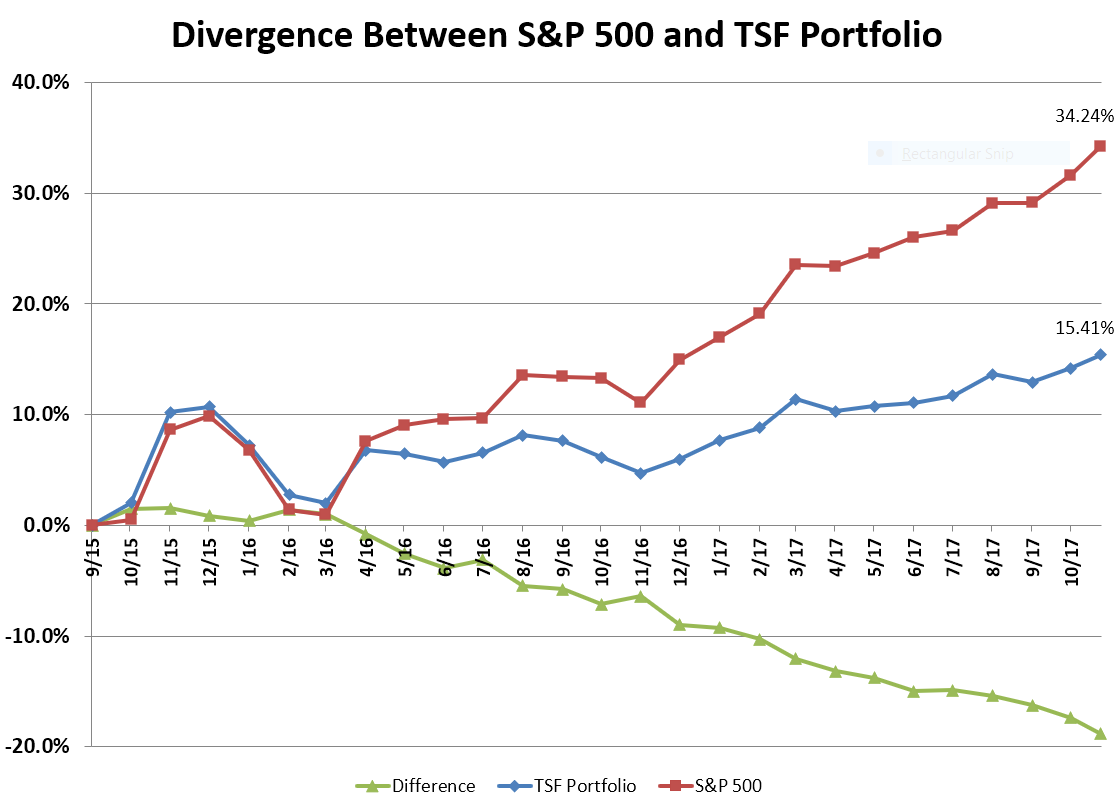
\includegraphics[width=.70\linewidth]{tsf_divergence.png}}
\end{center}

\end{enumerate}
Please reach out if you have any questions or comments regarding the portfolio. Thank you, \par
The Equity Strategy Team


\end{singlespace} % Uncomment for single line spacing


%----------------------------------------------------------------------------------------

\end{newlfm}
\end{document}
